%% ICNDEMAC-2027 -- Track 2: Nano-Electronics
%% IEEE conference paper (IEEEtran). Build with pdflatex (x2) + bibtex, or Overleaf.
\documentclass[conference]{IEEEtran}
\IEEEoverridecommandlockouts

\usepackage{cite}
\usepackage{amsmath,amssymb,amsfonts}
\usepackage{graphicx}
\usepackage{booktabs}
\usepackage{textcomp}
\usepackage{xcolor}
\usepackage[hidelinks]{hyperref}

\graphicspath{{figures/}}

\begin{document}

\title{A Self-Consistent Finite-Element Schr\"odinger--Poisson\\
Drift-Diffusion Solver for Quantum-Confinement Effects\\
in Ultra-Thin-Body Nanoscale Devices}

\author{%
\IEEEauthorblockN{Author One\IEEEauthorrefmark{1}, Author Two\IEEEauthorrefmark{2}}
\IEEEauthorblockA{\textit{Department of Electronics and Communication Engineering}\\
\textit{Affiliation, City, Country}\\
\IEEEauthorrefmark{1}email@domain \quad \IEEEauthorrefmark{2}email@domain}
}

\maketitle

\begin{abstract}
As field-effect transistors scale into the few-nanometre regime, the carriers in
the thin body occupy quantised subbands and the classical drift-diffusion (DD)
picture of a point-like charge continuum breaks down. We present an open-source,
two-dimensional finite-element device solver that couples the steady-state
drift-diffusion equations, written in the quasi-Fermi-potential variables and
solved by a fully-coupled Newton method with an exact analytic Jacobian, to a
self-consistent Schr\"odinger--Poisson (S--P) quantum-confinement correction. The
single-band effective-mass Schr\"odinger equation is solved slice-by-slice across
the confinement direction, and the resulting subband density enters the
drift-diffusion assembly as a charge-conserving additive quantum potential, so
the analytic Jacobian and the quadratic convergence of the inner Newton solve are
preserved. Using a silicon ultra-thin-body $p$--$n$ junction we show that the
ground-state subband spacing rises from $10$~meV at a $12$~nm body to $161$~meV at
$3$~nm, crossing the room-temperature thermal energy $k_BT$ near an
$8$~nm body---the onset of strong quantum confinement. The correction redistributes
carriers across the body by up to $\sim\!19\%$ while conserving charge to
$1.6\times10^{-5}$, leaves the ideal-diode terminal current essentially unchanged
(within $0.01\%$, ideality factor $\approx1.16$), and recovers the classical
solver exactly when disabled. Metal--oxide--semiconductor gate control
(accumulation $\rightarrow$ depletion $\rightarrow$ inversion) is reproduced on
the same framework. The solver is validated against analytic semiconductor
physics and provides a compact, extensible platform for quantum-corrected TCAD of
scaled nanoelectronic devices.
\end{abstract}

\begin{IEEEkeywords}
Schr\"odinger--Poisson, drift-diffusion, finite-element method, quantum
confinement, ultra-thin-body, TCAD, nanoelectronics, coupled Newton.
\end{IEEEkeywords}

\section{Introduction}
\IEEEPARstart{T}{he} continued scaling of CMOS technology into ultra-thin-body
silicon-on-insulator (UTB-SOI), FinFET and gate-all-around geometries places
device dimensions on the order of the electron de Broglie wavelength. In such
bodies the transverse motion of carriers is quantised into subbands: the charge
peak is set back from the confining walls, the lowest allowed energy is raised,
and the electrostatics that determine threshold voltage and inversion-layer
capacitance depart from the classical prediction~\cite{ando1982,sternhoward}.
Technology computer-aided design (TCAD) for such devices therefore needs a
quantum-corrected transport model that remains numerically robust and
inexpensive enough for routine use.

The drift-diffusion (DD) system~\cite{selberherr} remains the workhorse of device
simulation, but on its own it treats carriers as a point-like continuum whose
density follows the electrostatic potential instantaneously. A widely used and
computationally attractive remedy is to retain the DD transport equations along
the device while adding a self-consistent Schr\"odinger--Poisson (S--P) correction
that captures confinement across the thin dimension~\cite{sternhoward,trellakis}.
This paper presents a compact, open-source implementation of exactly this
strategy on an unstructured finite-element mesh, and characterises the resulting
quantum corrections for scaled silicon devices.

\textit{Contributions.} (i) A two-dimensional, finite-element,
quasi-Fermi-potential DD solver with a fully-coupled Newton scheme built on the
exact analytic $9\times9$ element Jacobian; (ii) a self-consistent, charge-conserving
S--P correction that enters the DD assembly as an additive quantum potential and
therefore leaves the inner Jacobian---and its quadratic convergence---unchanged;
(iii) a quantitative study of quantum-confinement scaling in silicon
ultra-thin-body junctions, and a demonstration of MOS gate control on the same
framework; and (iv) validation against analytic semiconductor physics.

\section{Numerical Formulation}

\subsection{Drift-diffusion core}
The steady state is described by the three coupled equations for the normalised
electrostatic potential $u=\psi/V_T$ and the electron and hole quasi-Fermi
potentials $v=\phi_n/V_T$, $w=\phi_p/V_T$, using De Mari intrinsic
scaling~\cite{demari} so that every unknown is $O(1)$. Carrier densities follow
algebraically from Boltzmann statistics, $n=n_i e^{\,u-v}$ and $p=n_i e^{\,w-u}$.
With $N_i$ the linear (P1) triangle shape functions and $C=(N_D-N_A)/n_i$ the
scaled net doping, the Galerkin weak forms are
\begin{align}
R_i^{u} &= \int_\Omega\!\big(\nabla N_i\!\cdot\!\nabla u + N_i(n-p-C)\big)\,d\Omega,\\
R_i^{v} &= \int_\Omega \mu_n\,n\,\nabla N_i\!\cdot\!\nabla v\;d\Omega,\\
R_i^{w} &= \int_\Omega \mu_p\,p\,\nabla N_i\!\cdot\!\nabla w\;d\Omega,
\end{align}
expressing Poisson's equation and the two zero-divergence continuity equations
$\nabla\!\cdot\!\mathbf{J}_n=\nabla\!\cdot\!\mathbf{J}_p=0$. Element integrals use
3-point Gauss quadrature on the reference triangle. The global $3N\times3N$ system
is solved by a damped Newton method using the exact analytic element Jacobian,
whose block structure is
\begin{equation}
J=\begin{bmatrix} K_{uu} & K_{uv} & K_{uw}\\ K_{vu} & K_{vv} & 0\\ K_{wu} & 0 & K_{ww}\end{bmatrix},
\end{equation}
with, e.g., $(K_{uu})_{ik}=\int\nabla N_i\!\cdot\!\nabla N_k\,d\Omega
+\int N_iN_k\big(e^{u-v}+e^{w-u}\big)\,d\Omega$. Per-step damping caps the largest
increment so the exponential density terms cannot overflow from a cold start.
Optional Shockley--Read--Hall and Auger recombination, per-region
heterojunction band offsets (Anderson's rule), Fermi--Dirac statistics, and
insulator/gate (MOS) and Schottky contacts are supported but are secondary to
the quantum correction studied here.

\subsection{Self-consistent Schr\"odinger--Poisson correction}
Confinement in a thin body is a one-dimensional effect across the thin dimension.
As in standard device TCAD, the mesh is cut into slices along the confinement
direction and, on each slice, the single-band effective-mass problem is solved by
linear finite elements:
\begin{equation}
\Big[-\frac{\hbar^2}{2m^*}\frac{d^2}{dy^2}+U(y)\Big]\psi_i(y)=E_i\,\psi_i(y),
\end{equation}
with $U_n(y)=-k_BT\,u(y)$ for electrons (and $U_p=+k_BT\,u$ for holes). The
tridiagonal generalised problem $H\psi=E\,M\psi$ (stiffness plus potential matrix,
consistent mass $M$) yields the lowest \texttt{num\_states} $M$-normalised
eigenpairs, summed with a thermal (Boltzmann) subband occupation
$g_i=e^{-(E_i-E_0)/k_BT}$ into the quantum density shape
$\rho(y)=\sum_i g_i|\psi_i(y)|^2$. This shape is renormalised so each slice carries
\emph{exactly the same charge} as the classical density it replaces; the
correction therefore only redistributes carriers across the confinement direction,
keeping Poisson's equation well posed. It enters the DD assembly as an additive
quantum potential $\Lambda$ in the density exponent,
\begin{equation}
n=n_i\,e^{\,u-v+\Lambda_n},\qquad \Lambda=\ln\!\frac{n_{\mathrm{QM}}}{n_{\mathrm{cl}}}.
\end{equation}
Because $\Lambda$ is held fixed within a Newton solve, the analytic Jacobian is
unchanged ($\partial n/\partial u=n$, etc.) and quadratic convergence is retained.
An outer Schr\"odinger--Poisson (Gummel) loop recomputes $\Lambda$ from the updated
potential, under-relaxes it, and iterates to a tolerance; with $\Lambda\equiv0$ the
scheme reproduces the classical solver bit-for-bit. This is a self-consistent
predictor--corrector S--P scheme with quasi-equilibrium subbands quantised across
one direction and transported classically along the device; it is not a full
non-equilibrium (NEGF) quantum-transport model.

\section{Results and Discussion}
All results use a silicon $p$--$n$ junction, $200$~nm long along transport
($N_A=N_D=10^{15}\,\mathrm{cm^{-3}}$), with the body thickness $t_b$ across the
confinement direction as the scaling variable; material parameters (permittivity,
affinity, gap, mobilities, effective masses) are read from an editable material
file. The $5$~nm reference device has $833$ nodes / $1536$ triangles; a full
bias sweep runs in $9.7$~s (classical) and $15.2$~s (S--P) on a single core.

\subsection{Validation against analytic physics}
The classical core reproduces textbook junction physics: the built-in potential
matches $V_{bi}=V_T\ln(N_AN_D/n_i^2)$, the law of mass action $np=n_i^2$ holds at
equilibrium to machine precision, the forward $I$--$V$ is exponential with
ideality factor $\approx1$, and the currents extracted at the two contacts are
equal and opposite (conservation). Enabling the S--P correction leaves all
equilibrium identities intact because the per-slice renormalisation is
charge-conserving.

\subsection{Quantum-confinement scaling}
Fig.~\ref{fig:scaling} shows the ground-state subband spacing $E_1-E_0$ as the
body is thinned. It rises steeply---following the expected
$\sim\!t_b^{-2}$ particle-in-a-box trend---from $10.1$~meV at $t_b=12$~nm to
$22.7$~meV at $8$~nm, $58.0$~meV at $5$~nm, and $161.2$~meV at $3$~nm
(Table~\ref{tab:scaling}). The spacing crosses the room-temperature thermal
energy $k_BT=25.9$~meV near $t_b\approx8$~nm: below this thickness a single
subband dominates the occupation and quantum confinement is strong, whereas above
it many subbands are thermally populated and the body behaves quasi-classically.
This crossover is the practical boundary at which a quantum correction becomes
mandatory for accurate electrostatics. Fig.~\ref{fig:ladder} shows the computed
electron subband ladder for the $5$~nm device; the eigenvalues are correctly
ordered and widely spaced relative to $k_BT$.

\begin{figure}[!t]
\centering
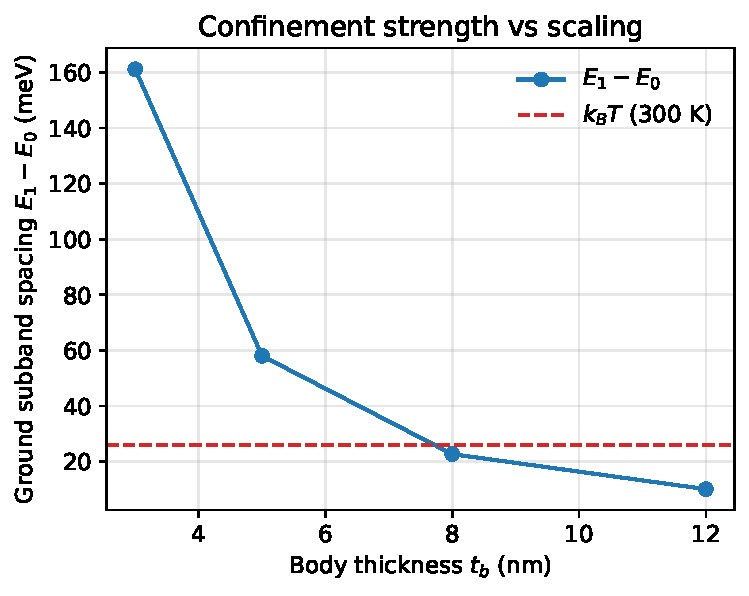
\includegraphics[width=\columnwidth]{fig_subband_vs_thickness.pdf}
\caption{Ground-state subband spacing $E_1-E_0$ versus silicon body thickness.
Confinement crosses the thermal energy $k_BT$ (300~K) near an $8$~nm body,
marking the onset of strong quantum confinement.}
\label{fig:scaling}
\end{figure}

\begin{table}[!t]
\caption{Confinement scaling in the silicon ultra-thin body}
\label{tab:scaling}
\centering
\begin{tabular}{cccc}
\toprule
$t_b$ (nm) & $E_1-E_0$ (meV) & $(E_1-E_0)/k_BT$ & regime\\
\midrule
12 & 10.1  & 0.39 & quasi-classical\\
 8 & 22.7  & 0.88 & crossover\\
 5 & 58.0  & 2.25 & confined\\
 3 & 161.2 & 6.24 & strongly confined\\
\bottomrule
\end{tabular}
\end{table}

\begin{figure}[!t]
\centering
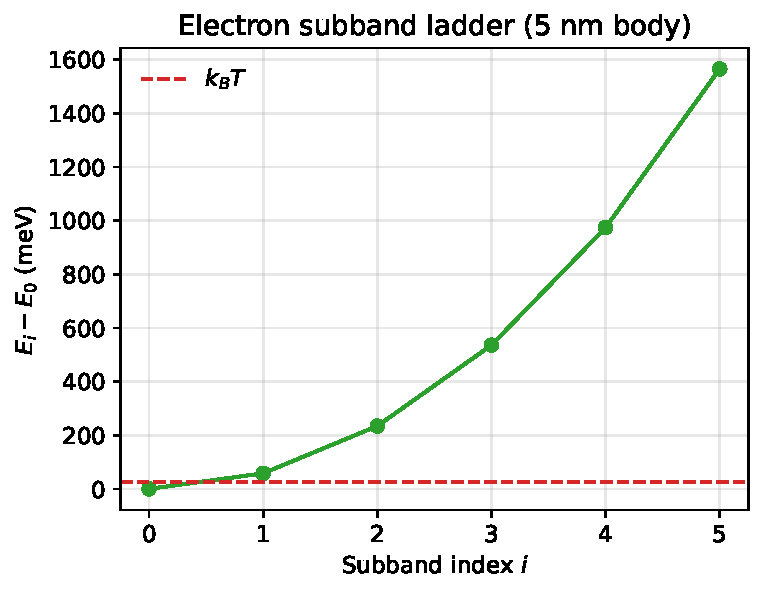
\includegraphics[width=\columnwidth]{fig_subbands.pdf}
\caption{Electron subband ladder (energies relative to the ground state) for the
$5$~nm body. The ground-to-first spacing is $58$~meV, well above $k_BT$.}
\label{fig:ladder}
\end{figure}

\subsection{Charge-conserving redistribution and terminal current}
Because the transverse electrostatic field is weak in a symmetric junction, the
classical transverse density profile is essentially flat. The S--P correction
modulates it by up to $19\%$ (Fig.~\ref{fig:redist}) while conserving the
slice charge to a relative error of $1.6\times10^{-5}$: the quantum potential
$\Lambda_n$ spans $[-0.10,+0.10]$ for the $5$~nm body. This redistribution is
precisely the quantum electrostatics that shifts inversion-layer capacitance in a
gated device. In the ungated diode, however, the terminal $I$--$V$ is left almost
unchanged: the extracted ideality factor is $1.16$ both with and without the
correction, and the forward current agrees to within $0.01\%$ over
$0.4$--$0.8$~V (Fig.~\ref{fig:iv}). This cleanly separates the two roles of the
correction---a first-order effect on the charge distribution and capacitance, but
a negligible effect on the ideal-diffusion current of an unconfined-transport
junction---and confirms that the coupled solve remains rectifying and
current-conserving with quantum physics enabled.

\begin{figure}[!t]
\centering
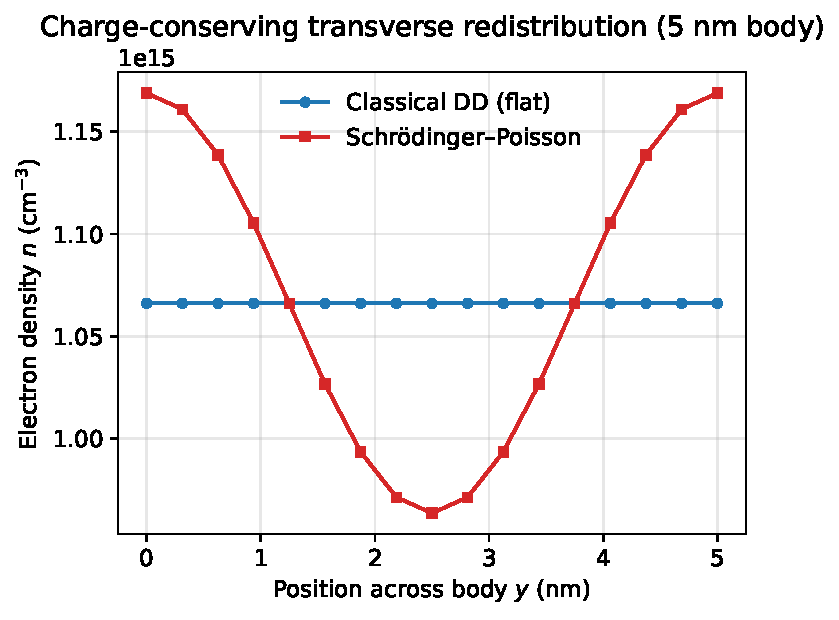
\includegraphics[width=\columnwidth]{fig_transverse_redistribution.pdf}
\caption{Electron density across the $5$~nm body (n-side slice). The classical
profile is flat; the charge-conserving Schr\"odinger--Poisson correction
redistributes carriers transversely by up to $19\%$.}
\label{fig:redist}
\end{figure}

\begin{figure}[!t]
\centering
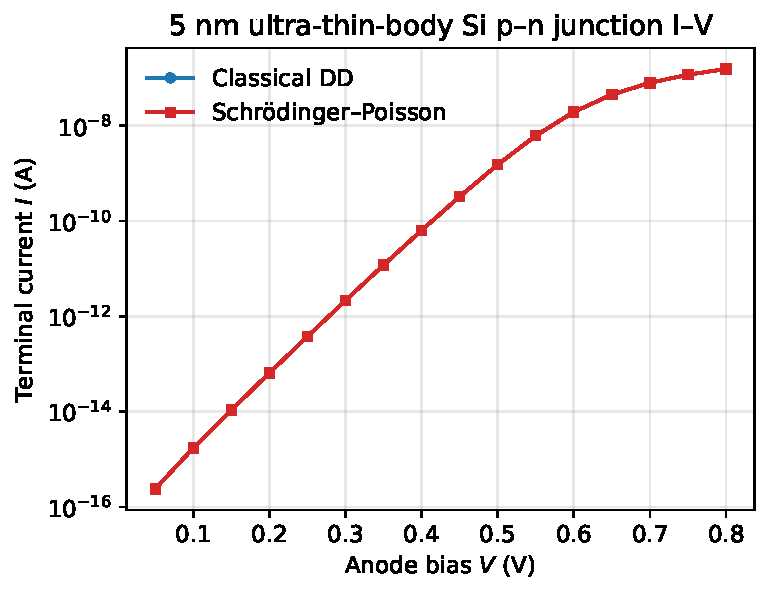
\includegraphics[width=\columnwidth]{fig_iv_classical_vs_quantum.pdf}
\caption{Forward $I$--$V$ of the $5$~nm ultra-thin-body junction. The quantum
correction preserves the ideal-diode current (ideality $\approx1.16$; agreement
within $0.01\%$), isolating its effect to the charge distribution.}
\label{fig:iv}
\end{figure}

\subsection{MOS gate control}
The same framework supports insulator (oxide) regions carrying permittivity but
no mobile charge, and an insulated metal-gate contact referenced through its work
function. Fig.~\ref{fig:mos} sweeps the gate of a
silicon/SiO\textsubscript{2} capacitor ($N_A=10^{17}\,\mathrm{cm^{-3}}$,
$t_{ox}=3$~nm): the silicon surface passes through accumulation
(surface holes $5.2\times10^{19}\,\mathrm{cm^{-3}}$), depletion, and strong
inversion (surface electrons $1.5\times10^{20}\,\mathrm{cm^{-3}}$), an
inversion-to-depletion electron ratio exceeding $10^{11}$. This confirms that the
solver captures the gate electrostatics of the MOS building block, onto which the
quantum inversion-layer correction of the previous sections directly applies.

\begin{figure}[!t]
\centering
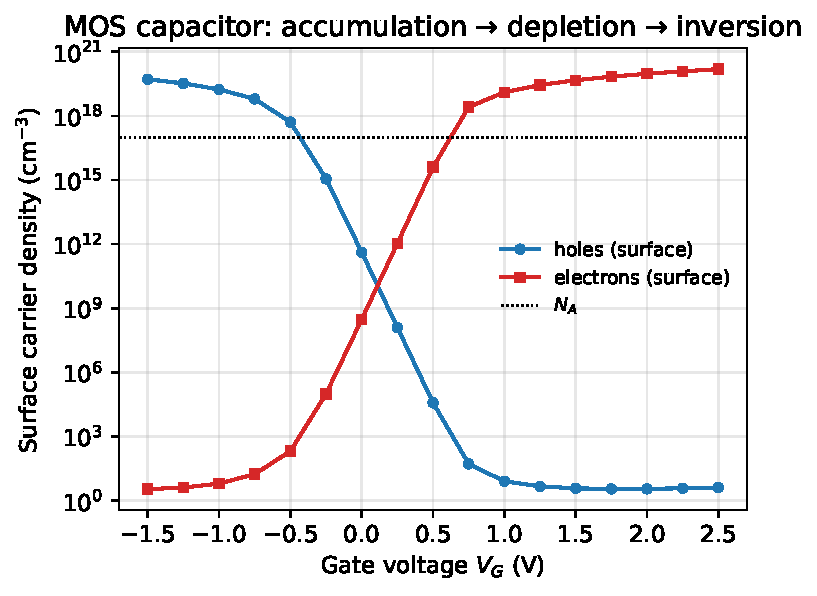
\includegraphics[width=\columnwidth]{fig_mos_gatecontrol.pdf}
\caption{MOS capacitor surface carrier densities versus gate voltage:
accumulation $\rightarrow$ depletion $\rightarrow$ inversion, reproduced on the
same finite-element framework.}
\label{fig:mos}
\end{figure}

\subsection{Discussion}
The correction is built and normalised per slice, so it is bounded and stable,
and is strongest exactly where it should be---thin, strongly-confined
bodies---fading as the body thickens and the subband spacing drops below $k_BT$,
consistent with Fig.~\ref{fig:scaling}. Slices are exact on structured/aligned
meshes; on a fully unstructured mesh, slices that cannot be formed are left
classical. Because the quantum potential enters as a frozen additive shift, the
method adds only an outer fixed-point loop around an otherwise unchanged
quadratically-convergent Newton solve---a favourable cost trade-off for routine
TCAD. The present model is a quasi-equilibrium, single-band scheme; multi-band
$k\!\cdot\!p$ subbands, thermionic-emission heterointerface transport, and
polarisation charge for wide-gap devices are natural extensions.

\section{Conclusion}
We have presented and validated an open-source, finite-element, self-consistent
Schr\"odinger--Poisson drift-diffusion solver for quantum-confinement effects in
scaled nanoelectronic devices. The coupled Newton core retains an exact analytic
Jacobian and quadratic convergence, and the charge-conserving quantum correction
adds only an outer loop. For silicon ultra-thin bodies the ground subband spacing
crosses $k_BT$ near $8$~nm, delimiting the strong-confinement regime; the
correction redistributes carriers by up to $19\%$ with negligible impact on the
ideal-diode current, and MOS gate control is reproduced on the same platform. The
tool offers a compact, extensible basis for quantum-corrected simulation of
emerging nanoscale devices.

\section*{Software and Reproducibility}
The solver and every example used to generate the figures in this paper are
open-source (MIT licence). All results were produced with the bundled
structured-mesh device demonstrations.

\begin{thebibliography}{1}
\bibitem{selberherr} S.~Selberherr, \emph{Analysis and Simulation of Semiconductor
Devices}. Vienna: Springer-Verlag, 1984.
\bibitem{ando1982} T.~Ando, A.~B.~Fowler, and F.~Stern, ``Electronic properties of
two-dimensional systems,'' \emph{Rev. Mod. Phys.}, vol.~54, no.~2, pp.~437--672, 1982.
\bibitem{sternhoward} F.~Stern and W.~E.~Howard, ``Properties of semiconductor
surface inversion layers in the electric quantum limit,'' \emph{Phys. Rev.},
vol.~163, no.~3, pp.~816--835, 1967.
\bibitem{demari} A.~De Mari, ``An accurate numerical steady-state one-dimensional
solution of the p-n junction,'' \emph{Solid-State Electron.}, vol.~11, no.~1,
pp.~33--58, 1968.
\bibitem{trellakis} A.~Trellakis, A.~T.~Galick, A.~Pacelli, and U.~Ravaioli,
``Iteration scheme for the solution of the two-dimensional Schr\"odinger--Poisson
equations in quantum structures,'' \emph{J. Appl. Phys.}, vol.~81, no.~12,
pp.~7880--7884, 1997.
\bibitem{irds} International Roadmap for Devices and Systems (IRDS), ``More Moore,''
IEEE, 2022.
\end{thebibliography}

\end{document}
